% [page size, font size, recto-verso]{style of the document}
\documentclass[a4paper, 12pt, oneside]{report}

% Encoding of this file. On Linux, all files are UTF8 encoded.
\usepackage[utf8x]{inputenc}

%Used to make nice looking listings:
\usepackage{listings}

% To write mathematical formula:
% \begin{align} ... \end{align}, \begin{equation} ... \end{equation}
\usepackage{amsmath, amssymb}

% To insert graphics:
% \includegraphics[options]{path}
\usepackage{graphicx}

% The allowed type of image files.
\DeclareGraphicsExtensions{.pdf, .png}

% To include code file without any layout
% \verbatiminput{path}
\usepackage{verbatim}

% To include PDF files
% \includepdf[pages = z,x-y]{path}
\usepackage{pdfpages}

% To do tables on many pages
% \begin{longtable}{define the columns} ... \end{longtable}
\usepackage{longtable}


\textwidth=16cm
\oddsidemargin=0pt
\evensidemargin=0pt

%% The 3 variables which you must initialize:
% Title of the document,
\newcommand{\titleVariable}{Obstacle Avoidance}
% The author(s),
\newcommand{\authorVariable}{Rik Smit}
% The date of the first release.
\newcommand{\firstRelease}{}

\usepackage{hyperref}
% To create all hypertext links for the bibliography, the figures, the bookmarks etc.
% \url{http://www.thewebsite.org}
\hypersetup{
%   backref=true,
%   pagebackref=true,
%   hyperindex=true,
    colorlinks=true,
    breaklinks=true,
    urlcolor= blue,
    linkcolor= blue,
%   bookmarks=true,
    bookmarksopen=true,
    pdftitle={\titleVariable},
    pdfauthor={\authorVariable},
    pdfsubject={Documentation}
}

\title{\titleVariable}
\author{\authorVariable}


\date{\centering First release: \firstRelease \\ Last modification: \today}

\begin{document}
\maketitle

\chapter{Obstacle Avoidance}

This document explains how to use the obstacle avoidance in the architecture. 
Also see the document ``Obstacle Detector'' on how to use the actual detector.

De obstacle avoider module makes sure the robot can avoid obstacles. 
It uses the obstacle matrix in memory created by the obstacle detector. 
Given this obstacle matrix in combination with a target vector (that points to the location you want the robot to be) the obstacle avoider will calculate a goal vector wich descripes the final movement the robot should make to reach its goal safely without bumping into obstacles.

\begin{figure}[H]
    \centering
    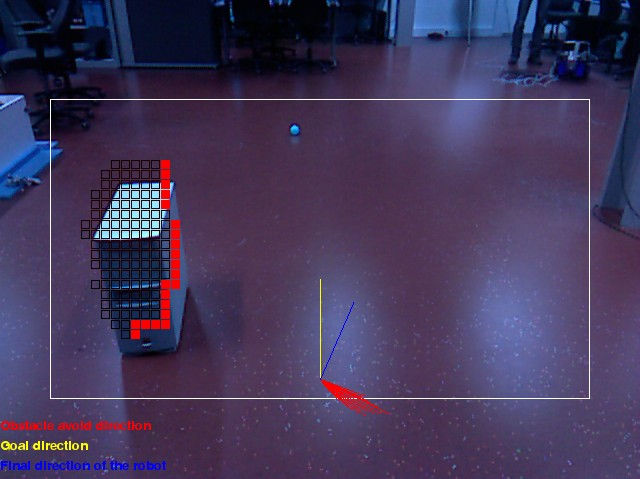
\includegraphics[width=0.9\textwidth]{../vision/img/obstacledetector_example.png}
    \caption{Screenshot of the obstacledetector module.\label{fig:example}}
\end{figure}

\section{The Scanned Obstacle Matrix}
For obstacle avoidance, a different obstacle matrix is used. 
The scanned obstacle matrix. 
This scanned obstacle matrix will contain only the edges of obstacles closest to the robot (filled squares in picture above). 
This is more useful for vector field navigation. 
In the picture above the scanned obstacle matrix will have the value 1 at the completely filled squares and the value 0 in all the other items.

\section{Using the Obstacle Avoider}
The obstacle avoider requires a target vector of the format (speed, angle). 
In the image above this is the yellow line. 
The target vector points at the at the place where you want the robot to be. 
The speed determines how fast you want the robot to go (range 0 to 1). 
The angle is in the range from -180 (right behind the robot) to 180 (also right behind the robot). 
-90 and 90 degrees are respectively to the left and the right of the robot and 0 is right in front of the robot.  
For example, you want to follow a person that is located at 30 degreest to the right of you, then the target vector will be (1,30) if you want to go there as fast as possible. 
The result of the obstacle avoider is a goal vector that specifies the real direction and speed for the robot. 
This is the blue line in the image above. 
If there are no obstacles spotted, the goal vector will be the same as the target vector. 
When there are obstacle spotted, the goal vector will generally pointing away from obstacles.

In the architecture, the obstacle avoider is used by the \lstinline{set_target} function of the pioneer. 
This function is used by modules to move the robot. 
Call it as \lstinline{set_target(target, False)} to let the robot move to a target , not using avoidance. 
Call it as \lstinline{set_target(target, True)} to let the robot move to a target and avoid obstacles at the same time.
The function should be called about 10 times per second to let the robot smoothly drive to the target. 
Ofcourse while continuously calling the function, you want to update the target vector as the target will move compared to the robot.

Since the obstacle avoider heavily depends on the obstacle detector and the Kinect, make sure that the obstacles detector is calibrated when the Kinect's position is changed.

\section{Vector Field Navigation}
The obstacle avoider uses vector field navigation. 
This method models the environment as a vector field. 
Every vector in that vector field tells the robot where to go when it is at that perticulair point in the environment. 
The calculation of the vectors is done in the vectorfield module. 
The obstacle avoider passes the obstacle matrix and the target vector to the vectorfield. 
From the obstacle matrix the vectorfield module will create obstacle vectors. 
This are the red lines in Image 1. 
The obstacle vectors point away from the obstacles, telling the robot to move away from them. 
All the obstacle vectors are summed, creating one general obstacle vector. 
This vector is then added to the specified target vector, creating one end vector, the goal vector.

\section{The Obstacle Vector}
In the vectorfield module the obstacle vectors are calculated from the obstacle matrix. 
First from every obstacle (item in the matrix) an initial obstacle vector is calculated from the format (length, direction). 
Then the obstacle affect vectors are calculated. 
These are the vectors that will eventually influence the robot movement. 
It is important that the function calculates the affect vectors is tuned well in order to not let the robot bumb into obstacles. 
First all obstacles at a certain distance are filtered out, so only obstacles close enough to the robot will influence the movement. 
Using a formula the final obstacle affect vectors are calculated. 
Currently this is an exponentional function that lets obstacles closer to the robot influence the robot exponentionally more the obstacles further away. 
In order to tune the obstacle avoider, the distance treshold should be adjusted as well as the formule that calculates the final obstacle (affect) vector.

\end{document}
